%%%%%%%%%%%%%%%%%%%%%%%%%%%%%%%%%%%%%%%%%%%%%%%%%%%%%%%%%%%%%%%%%%%%%
% Use the koma-script document style
\documentclass{scrbook}
%\KOMAoptions{twoside=false} % disable two-side formatting for scrbook
% alternatively, for shorter essay, use the following
% \documentclass{scrartcl}
%%%%%%%%%%%%%%%%%%%%%%%%%%%%%%%%%%%%%%%%%%%%%%%%%%%%%%%%%%%%%%%%%%%%%

%%%%%%%%%%%%%%%%%%%%%%%%%%%%%%%%%%%%%%%%%%%%%%%%%%%%%%%%%%%%%%%%%%%%%
% Useful packages
\usepackage{mathtools}
\usepackage{amssymb,bm,bbold}
\usepackage{enumerate}

\usepackage{hhline}
\usepackage{float}

% CSCI-265
\usepackage{tikz}
\usetikzlibrary{automata, positioning, arrows, arrows.meta}


%=================================
% pre-defined theorem environments
\usepackage{amsthm}
\newtheorem{theorem}{Theorem}
\newtheorem{lemma}{Lemma}
\newtheorem{proposition}{Proposition}
\newtheorem{corollary}{Corollary}
\newtheorem{definition}{Definition}
\newtheorem*{remark}{Remark}
\newtheorem*{assumption}{Assumption}

%=================================
% useful commands
\DeclareMathOperator*{\argmin}{arg\,min}
\DeclareMathOperator*{\argmax}{arg\,max}
\DeclareMathOperator*{\supp}{supp}

\def\vec#1{{\ensuremath{\bm{{#1}}}}}
\def\mat#1{\vec{#1}}

%=================================
% convenient notations
\newcommand{\XX}{\mathbb{X}}
\newcommand{\RR}{\mathbb{R}}
\newcommand{\NN}{\mathbb{N}}
\newcommand{\QQ}{\mathbb{Q}}
\newcommand{\ZZ}{\mathbb{Z}}
\newcommand{\EE}{\mathbb{E}}
\newcommand{\PP}{\mathbb{P}}

\newcommand{\sL}{\mathcal{L}}
\newcommand{\sX}{\mathcal{X}}
\newcommand{\sY}{\mathcal{Y}}

\newcommand{\ind}{\mathbb{1}}

\newcommand{\kleene}{{}^\ast}

%%%%%%%%%%%%%%%%%%%%%%%%%%%%%%%%%%%%%%%%%%%%%%%%%%%%%%%%%%%%%%%%%%%%%
% Typography, change document font
\usepackage[tt=false, type1=true]{libertine}
\usepackage[varqu]{zi4}
\usepackage[libertine]{newtxmath}
\usepackage[T1]{fontenc}

\usepackage[protrusion=true,expansion=true]{microtype}

\author{Guy Matz}

\begin{document}
	
\tikzset{
	->, % makes the edges directed 
%		>='stealth', % makes the arrow heads bold 
	node distance=3cm, % specifies the minimum distance between two nodes. Change if necessary. 
	every state/.style={thick, fill=gray!10}, % sets the properties for each ’state’ node 
	initial text=$ $, % sets the text that appears on the start arrow 
}
	
\title{Title}
% \maketitle

% \tableofcontents
% 
% %\bibliography{bibfile}
% 
% \end{document}


\begin{enumerate}

\item \textbf{For the language $L$ over $\{a,b,c\}$ defined by the regular expression} $$(a+b)\kleene(b+c)\kleene(c+a)\kleene$$

\begin{enumerate}
    \item Find the shortest word not in $L$.
    $$cab$$
    \item Draw an $\epsilon$NFA that accepts $L$ informally (without using Thompson's Construction Algorithm).
\\  I don't think I lnow how to do this without Thompson's algorithm
    
    \item Draw a DFA that accepts $L$.

          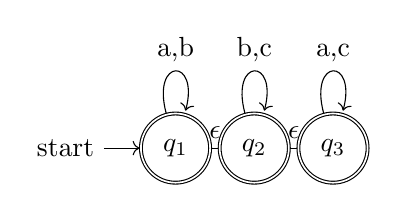
\begin{tikzpicture}
	\node[state, accepting, initial] (q1) {$q_1$};
	\node[state, accepting, right of=q1] (q2) {$q_2$};
	\node[state, accepting, right of=q2] (q3) {$q_3$};
	\draw
	
	(q1) edge[above] node{$\epsilon$} (q2)    	
	(q2) edge[above] node{$\epsilon$} (q3)
	
	(q1) edge[loop above] node{a,b} (q1)
	(q2) edge[loop above] node{b,c} (q2)    	
	(q3) edge[loop above] node{a,c} (q3)
	;
\end{tikzpicture}

\end{enumerate}

\newpage

\item \textbf{Convert the following to $\epsilon$NFAs, where $S1$, $S2$, and
    $S3$ are regular expressions that may be represented by a single
    transition from the start state to the sole accepting state of an
    $\epsilon$NFA that recognizes them (this means you may treat them like
    single letters as long as you use Thompson's Construction Algorithm correctly).}

\begin{enumerate}
    \item $S_1 S_2 S_3$
        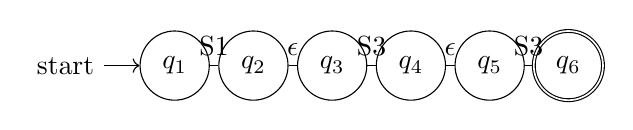
\begin{tikzpicture}
	\node[state, initial] (q1) {$q_1$};
	\node[state,  right of=q1] (q2) {$q_2$};
	\node[state,  right of=q2] (q3) {$q_3$};
	\node[state,  right of=q3] (q4) {$q_4$};
		\node[state,  right of=q4] (q5) {$q_5$};
	\node[state, accepting, right of=q5] (q6) {$q_6$};
	\draw
	
	(q1) edge[above] node{S1} (q2)
	(q2) edge[above] node{$\epsilon$} (q3)
	(q3) edge[above] node{S3} (q4)	
(q4) edge[above] node{$\epsilon$} (q5)
(q5) edge[above] node{S3} (q6)	

	;
\end{tikzpicture}


    \item $S_1 S_2 \kleene S_3$
            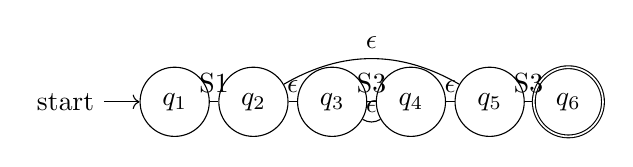
\begin{tikzpicture}
    	\node[state, initial] (q1) {$q_1$};
    	\node[state,  right of=q1] (q2) {$q_2$};
    	\node[state,  right of=q2] (q3) {$q_3$};
    	\node[state,  right of=q3] (q4) {$q_4$};
    	\node[state,  right of=q4] (q5) {$q_5$};
    	\node[state, accepting, right of=q5] (q6) {$q_6$};
    	\draw
    	
    	(q1) edge[above] node{S1} (q2)
    	(q2) edge[above] node{$\epsilon$} (q3)
    	(q3) edge[above] node{S3} (q4)	
    	(q4) edge[above] node{$\epsilon$} (q5)
    	(q5) edge[above] node{S3} (q6)	
    	
        (q2) edge[bend left, above] node{$\epsilon$} (q5)
        (q4) edge[bend left, above] node{$\epsilon$} (q3)
    	
    	;
    \end{tikzpicture}

    \item $S_1 + S_2$
            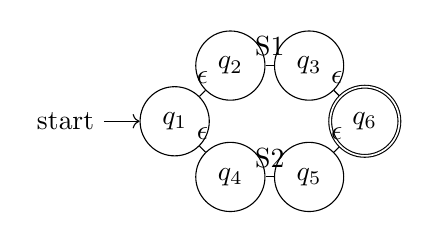
\begin{tikzpicture}
    	\node[state, initial] (q1) {$q_1$};
    	\node[state,  above right of=q1] (q2) {$q_2$};
    	\node[state,  right of=q2] (q3) {$q_3$};
    	\node[state,  below right of=q1] (q4) {$q_4$};
    	\node[state,  right of=q4] (q5) {$q_5$};
    	\node[state, accepting, above right of=q5] (q6) {$q_6$};
    	\draw
    	
    	(q1) edge[above] node{$\epsilon$} (q2)
    	(q1) edge[above] node{$\epsilon$} (q4)
    	(q2) edge[above] node{S1} (q3)
    	(q3) edge[above] node{$\epsilon$} (q6)	
    	(q4) edge[above] node{S2} (q5)
    	(q5) edge[above] node{$\epsilon$} (q6)	
    	
    	;
    \end{tikzpicture}
\end{enumerate}

\newpage

\item \textbf{Draw out the NFA from question 2 part b fully,
    using:}
     $$S_1 = ab+ba;  S_2 = aa+b(bb)\kleene ;S3 = b\kleene (a+ \epsilon)$$
\\\\
        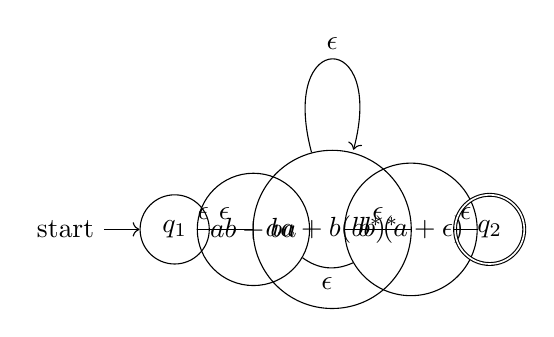
\begin{tikzpicture}
	\node[state, initial] (q1) {$q_1$};
	\node[state,  right of=q1] (s1) {$ab + ba$};
	\node[state,  right of=s1] (s2) {$aa + b(bb)\kleene$};
	\node[state,  right of=s2] (s3) {$b\kleene (a + \epsilon)$};
	\node[state, accepting, right of=s3] (q2) {$q_2$};
	\draw
	
	(q1) edge[above] node{$\epsilon$} (s1)
	(s1) edge[above] node{$\epsilon$} (s2)
	
	(s2) edge[loop above] node{$\epsilon$} (s2)
	(s3) edge[bend left, below] node{$\epsilon$} (s1)
	(s2) edge[above] node{$\epsilon$} (s3)
	(s3) edge[above] node{$\epsilon$} (q2)
	
	;
\end{tikzpicture}

\newpage
\item \textbf{Prove or disprove each of the following:}

\begin{enumerate}
    \item $L1 = \{ab, aab, bbb, aabaa\}$ is regular.
    \\\\ True since all finite languages are regular,  as they can all be expressed by a regular expression.
    \\
    \item Every finite language is regular. Hint: Consider the explicit definition of a set. Apply that to finite languages, and write a constructive proof that creates a regular expression for any given finite language that is expressed explicitly.
    \\\\
    As above, since every Finite Language can be expressed as a regular expression, every finite language is regular

\end{enumerate}

\newpage
\item \textbf{Write "every finite language is regular" as a first-order formula, and find its complement, contrapositive, and dual. Express each of those as both a first-order formula and a written description in English.}
\\\\Let $R(x)$ be "$x$ Regular Language", and let $F(x)$ be "$x$ is a Finite Language" and let $L$ be the set of all Languages
\begin{itemize}
	\item First Order: All Finite languages are Regular
		$$\forall x \in L \, F(x) \implies R(x)$$
	\item Complement: Not all Finite Languages are Regular
		$$\neg \forall x \in L \, F(x) \implies R(x)$$
	\item Contrapositive: All non-regular languages are infinite
	    $$ \forall x \in L \, \neg  R(x) \implies \neg  R(x)$$
	\item Dual: There are no Languages that are Finite but not Regular
		$$\neg \exists x \in L  \, ( F(x) \wedge \neg R(x) )$$
		
\end{itemize}


\newpage
\item \textbf{Explain why Thompson's Construction Algorithm is considered to be a proof by induction. Hint: consider what the inductive steps and base cases are. What does Thompson's Construction Algorithm prove?}
\\\\
Because it is an exhaustive proof

\newpage
\item \textbf{Construct both an NFA and a DFA which will recognize the language over $\{a,b\}$ consisting of all words where the third to last letter is "$b$" (meaning the letter two before the last letter). Then minimize your DFA (or confirm that it is already minimal).}
\\\\
$$(a + b) \kleene b (a + b) (a + b)$$

	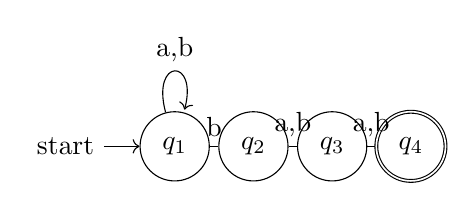
\begin{tikzpicture}
		\node[state, initial] (q1) {$q_1$};
		\node[state,  right of=q1] (q2) {$q_2$};
		\node[state,  right of=q2] (q3) {$q_3$};
		\node[state,  accepting, right of=q3] (q4) {$q_4$};
		\draw
    	(q1) edge[loop above] node{a,b} (q1)
		(q1) edge[above] node{b} (q2)
		(q2) edge[above] node{a,b} (q3)
		(q3) edge[above] node{a,b} (q4)	
		
		;
	\end{tikzpicture}
\end{enumerate}

% %\bibliography{bibfile}

\end{document}

